\documentclass{standalone}
\usepackage{tikz}
\usepackage{verbatim}
\usetikzlibrary{positioning}
\begin{document}
\pagestyle{empty}
  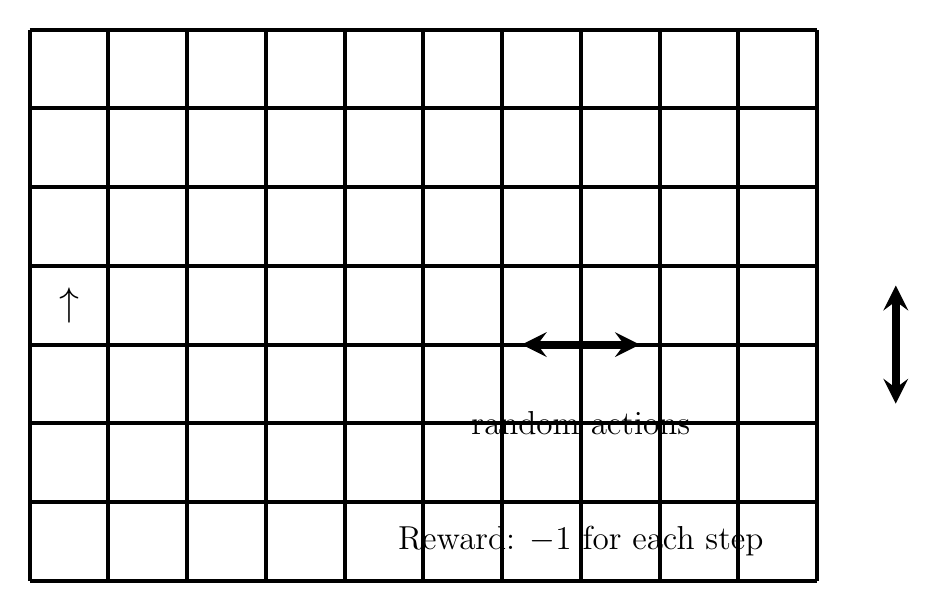
\begin{tikzpicture}
    \draw[stealth-stealth, line width=1 mm] (7.75, 3) -- (6.25, 3);
    \draw[stealth-stealth, line width=1 mm] (11, 2.25) -- (11, 3.75);
    \node at (7, 2) {\large random actions};
    \node at (7, 0.5) {\large Reward: $-1$ for each step};
    \node at (0.5, 3.5) {\Large $\uparrow$};


    \draw[step=1.0,black, line width=0.5 mm] (0,0) grid (10, 7);
  \end{tikzpicture}
\end{document}